\documentclass{standalone}
\usepackage{tikz}
\usetikzlibrary{patterns, positioning}


\begin{document}
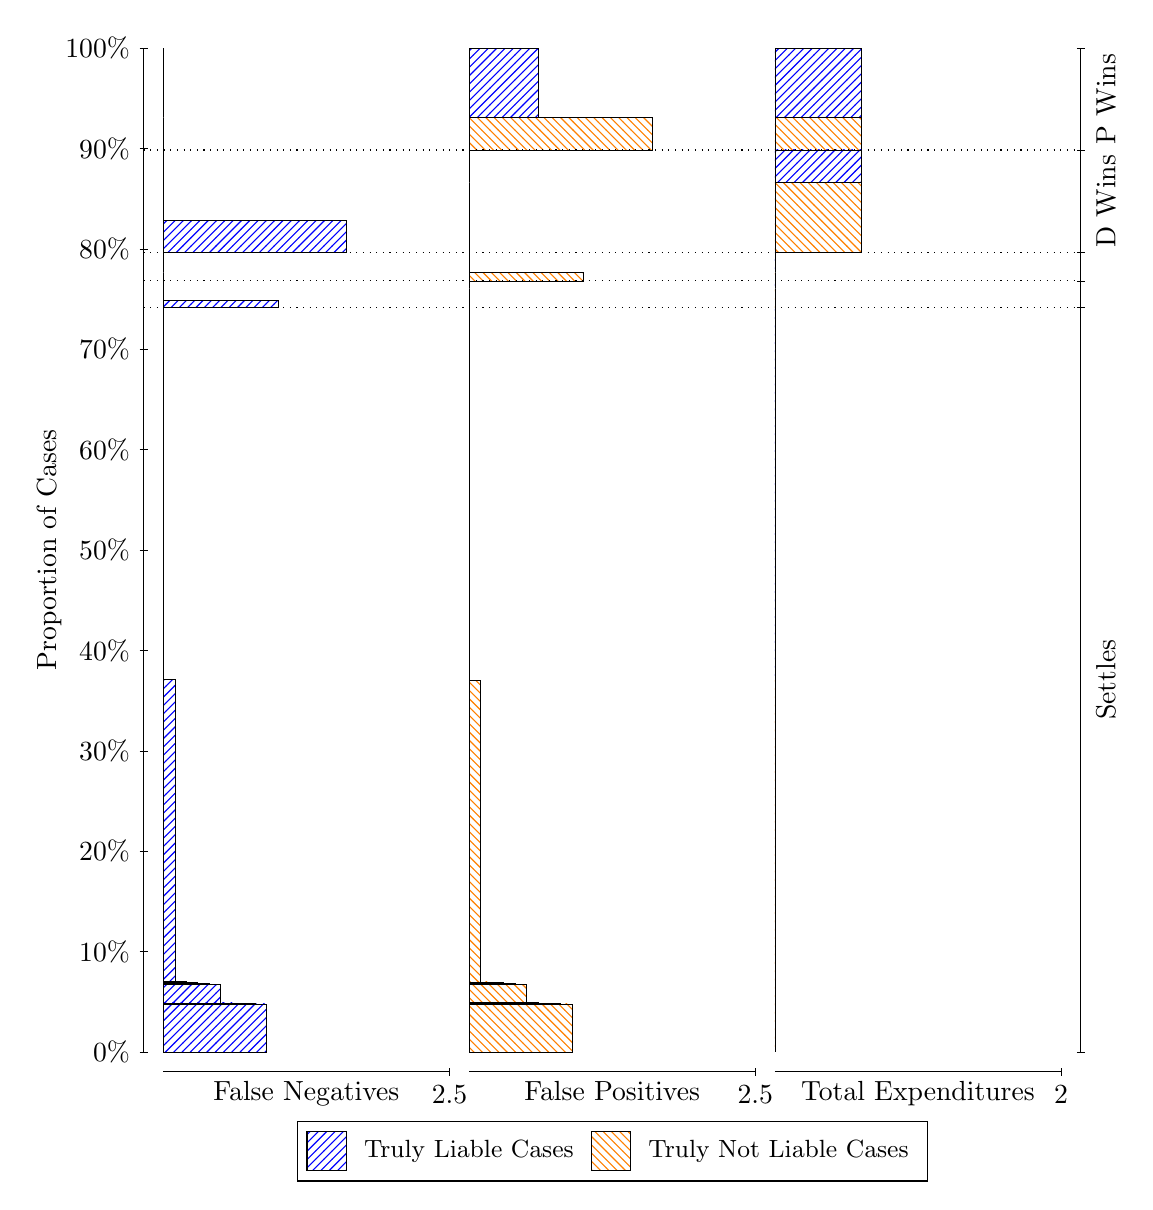
\begin{tikzpicture}
\draw[black, very thin] (1.5,1.75) -- (1.5,14.5);
\node[rotate=90, text=black, anchor=center] at (0.3, 8.125) {Proportion of Cases};
\draw[black, very thin] (1.45,1.75) -- (1.55,1.75);
\node[text=black, anchor=east] at (1.45, 1.75) {0\%};
\draw[black, very thin] (1.45,3.025) -- (1.55,3.025);
\node[text=black, anchor=east] at (1.45, 3.025) {10\%};
\draw[black, very thin] (1.45,4.3) -- (1.55,4.3);
\node[text=black, anchor=east] at (1.45, 4.3) {20\%};
\draw[black, very thin] (1.45,5.575) -- (1.55,5.575);
\node[text=black, anchor=east] at (1.45, 5.575) {30\%};
\draw[black, very thin] (1.45,6.85) -- (1.55,6.85);
\node[text=black, anchor=east] at (1.45, 6.85) {40\%};
\draw[black, very thin] (1.45,8.125) -- (1.55,8.125);
\node[text=black, anchor=east] at (1.45, 8.125) {50\%};
\draw[black, very thin] (1.45,9.4) -- (1.55,9.4);
\node[text=black, anchor=east] at (1.45, 9.4) {60\%};
\draw[black, very thin] (1.45,10.675) -- (1.55,10.675);
\node[text=black, anchor=east] at (1.45, 10.675) {70\%};
\draw[black, very thin] (1.45,11.95) -- (1.55,11.95);
\node[text=black, anchor=east] at (1.45, 11.95) {80\%};
\draw[black, very thin] (1.45,13.225) -- (1.55,13.225);
\node[text=black, anchor=east] at (1.45, 13.225) {90\%};
\draw[black, very thin] (1.45,14.5) -- (1.55,14.5);
\node[text=black, anchor=east] at (1.45, 14.5) {100\%};

\draw[black, very thin] (13.4,1.75) -- (13.4,14.5);
\draw[black, very thin] (13.35,1.75) -- (13.45,1.75);
\node[anchor=west] at (13.35, 1.75) {};
\draw[black, very thin] (13.35,11.204) -- (13.45,11.204);
\node[anchor=west] at (13.35, 11.204) {};
\draw[black, very thin] (13.35,11.542) -- (13.45,11.542);
\node[anchor=west] at (13.35, 11.542) {};
\draw[black, very thin] (13.35,11.901) -- (13.45,11.901);
\node[anchor=west] at (13.35, 11.901) {};
\draw[black, very thin] (13.35,13.205) -- (13.45,13.205);
\node[anchor=west] at (13.35, 13.205) {};
\draw[black, very thin] (13.35,14.5) -- (13.45,14.5);
\node[anchor=west] at (13.35, 14.5) {};

\draw[black, very thin, pattern color=blue, pattern=north east lines] (1.75,1.75) rectangle (3.058,2.3612);
\draw[black, very thin, pattern color=blue, pattern=north east lines] (1.75,2.3612) rectangle (2.9127,2.3651);
\draw[black, very thin, pattern color=blue, pattern=north east lines] (1.75,2.3651) rectangle (2.7673,2.3695);
\draw[black, very thin, pattern color=blue, pattern=north east lines] (1.75,2.3695) rectangle (2.622,2.3741);
\draw[black, very thin, pattern color=blue, pattern=north east lines] (1.75,2.3741) rectangle (2.622,2.3742);
\draw[black, very thin, pattern color=blue, pattern=north east lines] (1.75,2.3742) rectangle (2.4767,2.6067);
\draw[black, very thin, pattern color=blue, pattern=north east lines] (1.75,2.6067) rectangle (2.3313,2.6193);
\draw[black, very thin, pattern color=blue, pattern=north east lines] (1.75,2.6193) rectangle (2.186,2.632);
\draw[black, very thin, pattern color=blue, pattern=north east lines] (1.75,2.632) rectangle (2.0407,2.6447);
\draw[black, very thin, pattern color=blue, pattern=north east lines] (1.75,2.6447) rectangle (1.8953,6.4802);
\draw[black, very thin, pattern color=orange, pattern=north west lines] (1.75,6.4802) rectangle (1.75,11.204);
\draw[black, very thin, pattern color=blue, pattern=north east lines] (1.75,11.204) rectangle (3.2033,11.299);
\draw[black, very thin, pattern color=orange, pattern=north west lines] (1.75,11.299) rectangle (1.75,11.542);
\draw[black, very thin, pattern color=orange, pattern=north west lines] (1.75,11.542) rectangle (1.75,11.647);
\draw[black, very thin, pattern color=blue, pattern=north east lines] (1.75,11.647) rectangle (1.75,11.901);
\draw[black, very thin, pattern color=blue, pattern=north east lines] (1.75,11.901) rectangle (4.0753,12.312);
\draw[black, very thin, pattern color=orange, pattern=north west lines] (1.75,12.312) rectangle (1.75,13.205);
\draw[black, very thin, pattern color=orange, pattern=north west lines] (1.75,13.205) rectangle (1.75,13.615);
\draw[black, very thin, pattern color=blue, pattern=north east lines] (1.75,13.615) rectangle (1.75,14.5);
\draw[black, very thin, pattern color=orange, pattern=north west lines] (5.6333,1.75) rectangle (6.9413,2.3612);
\draw[black, very thin, pattern color=orange, pattern=north west lines] (5.6333,2.3612) rectangle (6.796,2.3664);
\draw[black, very thin, pattern color=orange, pattern=north west lines] (5.6333,2.3664) rectangle (6.6507,2.3717);
\draw[black, very thin, pattern color=orange, pattern=north west lines] (5.6333,2.3717) rectangle (6.5053,2.3769);
\draw[black, very thin, pattern color=orange, pattern=north west lines] (5.6333,2.3769) rectangle (6.36,2.6096);
\draw[black, very thin, pattern color=orange, pattern=north west lines] (5.6333,2.6096) rectangle (6.2147,2.6098);
\draw[black, very thin, pattern color=orange, pattern=north west lines] (5.6333,2.6098) rectangle (6.2147,2.621);
\draw[black, very thin, pattern color=orange, pattern=north west lines] (5.6333,2.621) rectangle (6.0693,2.6314);
\draw[black, very thin, pattern color=orange, pattern=north west lines] (5.6333,2.6314) rectangle (5.924,2.6409);
\draw[black, very thin, pattern color=orange, pattern=north west lines] (5.6333,2.6409) rectangle (5.7787,6.4737);
\draw[black, very thin, pattern color=blue, pattern=north east lines] (5.6333,6.4737) rectangle (5.6333,11.204);
\draw[black, very thin, pattern color=orange, pattern=north west lines] (5.6333,11.204) rectangle (5.6333,11.447);
\draw[black, very thin, pattern color=blue, pattern=north east lines] (5.6333,11.447) rectangle (5.6333,11.542);
\draw[black, very thin, pattern color=orange, pattern=north west lines] (5.6333,11.542) rectangle (7.0867,11.647);
\draw[black, very thin, pattern color=blue, pattern=north east lines] (5.6333,11.647) rectangle (5.6333,11.901);
\draw[black, very thin, pattern color=orange, pattern=north west lines] (5.6333,11.901) rectangle (5.6333,12.794);
\draw[black, very thin, pattern color=blue, pattern=north east lines] (5.6333,12.794) rectangle (5.6333,13.205);
\draw[black, very thin, pattern color=orange, pattern=north west lines] (5.6333,13.205) rectangle (7.9587,13.615);
\draw[black, very thin, pattern color=blue, pattern=north east lines] (5.6333,13.615) rectangle (6.5053,14.5);
\draw[black, very thin, pattern color=orange, pattern=north west lines] (9.5167,1.75) rectangle (9.5167,6.4737);
\draw[black, very thin, pattern color=blue, pattern=north east lines] (9.5167,6.4737) rectangle (9.5167,11.204);
\draw[black, very thin, pattern color=orange, pattern=north west lines] (9.5167,11.204) rectangle (9.5167,11.447);
\draw[black, very thin, pattern color=blue, pattern=north east lines] (9.5167,11.447) rectangle (9.5167,11.542);
\draw[black, very thin, pattern color=orange, pattern=north west lines] (9.5167,11.542) rectangle (9.5167,11.647);
\draw[black, very thin, pattern color=blue, pattern=north east lines] (9.5167,11.647) rectangle (9.5167,11.901);
\draw[black, very thin, pattern color=orange, pattern=north west lines] (9.5167,11.901) rectangle (10.607,12.794);
\draw[black, very thin, pattern color=blue, pattern=north east lines] (9.5167,12.794) rectangle (10.607,13.205);
\draw[black, very thin, pattern color=orange, pattern=north west lines] (9.5167,13.205) rectangle (10.607,13.615);
\draw[black, very thin, pattern color=blue, pattern=north east lines] (9.5167,13.615) rectangle (10.607,14.5);
\draw[black, dotted] (1.5,11.204) -- (13.4,11.204);
\draw[black, dotted] (1.5,11.542) -- (13.4,11.542);
\draw[black, dotted] (1.5,11.901) -- (13.4,11.901);
\draw[black, dotted] (1.5,13.205) -- (13.4,13.205);
\draw[black, very thin] (1.75,1.5) -- (5.3833,1.5);
\node[text=black, anchor=north] at (3.5667, 1.5) {False Negatives};
\draw[black, very thin] (5.3833,1.45) -- (5.3833,1.55);
\node[text=black, anchor=north] at (5.3833, 1.45) {2.5};

\draw[black, very thin] (5.6333,1.5) -- (9.2667,1.5);
\node[text=black, anchor=north] at (7.45, 1.5) {False Positives};
\draw[black, very thin] (9.2667,1.45) -- (9.2667,1.55);
\node[text=black, anchor=north] at (9.2667, 1.45) {2.5};

\draw[black, very thin] (9.5167,1.5) -- (13.15,1.5);
\node[text=black, anchor=north] at (11.333, 1.5) {Total Expenditures};
\draw[black, very thin] (13.15,1.45) -- (13.15,1.55);
\node[text=black, anchor=north] at (13.15, 1.45) {2};

\node[text=black, centered, rotate=90] at (13.72, 6.4769) {Settles};


\node[text=black, centered, rotate=90] at (13.72, 12.553) {D Wins};
\node[text=black, centered, rotate=90] at (13.72, 13.852) {P Wins};

\draw (7.449999999999999,1.5) node[draw=none] (baseCoordinate) {};
\begin{scope}[align=center]
        \matrix[scale=0.5, draw=black, below=0.5cm of baseCoordinate, nodes={draw}, column sep=0.1cm]{
            \node[rectangle, draw, minimum width=0.5cm, minimum height=0.5cm, pattern color=blue, pattern=north east lines] {}; &
            \node[draw=none, font=\small, text=black] (B) {Truly Liable Cases}; &
            \node[rectangle, draw, minimum width=0.5cm, minimum height=0.5cm, pattern color=orange, pattern=north west lines] {}; &
            \node[draw=none, font=\small, text=black] (B) {Truly Not Liable Cases}; \\
            };
\end{scope}

\end{tikzpicture}
\end{document}